\documentclass[10pt,a4paper]{article}

\usepackage[utf8]{inputenc}
\usepackage[T1]{fontenc}
\usepackage[brazil]{babel}
\usepackage{helvet}
\renewcommand{\familydefault}{\sfdefault}
\usepackage[top=16mm,bottom=18mm,left=15mm,right=15mm]{geometry}
\usepackage{xcolor}
\usepackage{graphicx}
\usepackage{booktabs}
\usepackage{tabularx}
\usepackage{array}
\usepackage{colortbl}
\usepackage{multicol}
\usepackage{lettrine}
\usepackage{fancyhdr}
\usepackage{lastpage}
\usepackage{hyperref}
\usepackage{parskip}

% ==============================================================================
% PALETA HARMONICA DINAMICA (INJETADA PELO R CONFORME CARTA OU DOSSIE)
% Mantem o Dourado Institucional (#C8942B) como DNA do Jornal Economico do TO
% ==============================================================================
\definecolor{corprimaria}{HTML}{12352B}
\definecolor{corsecundaria}{HTML}{2A6F57}
\definecolor{douradoto}{HTML}{C8942B}
\definecolor{corfundo}{HTML}{F2F7F5}
\definecolor{cinzatexto}{HTML}{262D33}
\definecolor{cinzasuave}{HTML}{5A6570}
\definecolor{borda}{HTML}{D5DCE2}

\hypersetup{
    colorlinks=true,
    linkcolor=corprimaria,
    urlcolor=douradoto,
    pdftitle={Carta de Conjuntura do Tocantins: Descolamento positivo do PIB estadual e resiliência do setor de serviços},
    pdfauthor={Lorenzo Costa e Equipe | Núcleo de Conjuntura do Jornal Econômico do Tocantins}
}

\setlength{\parindent}{0pt}
\setlength{\parskip}{5pt}
\renewcommand{\arraystretch}{1.24}

% Configuracao do formato de Periodico / Revista (2 Colunas)
\setlength{\columnsep}{18pt}
\setlength{\columnseprule}{0.4pt}
\renewcommand{\columnseprulecolor}{\color{borda}}

% Cabecalho e Rodape de Periodico
\pagestyle{fancy}
\fancyhf{}
\renewcommand{\headrulewidth}{0pt}
\renewcommand{\footrulewidth}{0.8pt}
\renewcommand{\footrule}{\hbox to\headwidth{\color{douradoto}\leaders\hrule height \footrulewidth\hfill}}

\fancyfoot[L]{\footnotesize\textcolor{corprimaria}{\textbf{JORNAL ECONÔMICO DO TOCANTINS}} \textcolor{cinzasuave}{$\vert$ CARTA DE CONJUNTURA ECONÔMICA $\bullet$ 3º Trimestre de 2026}}
\fancyfoot[R]{\footnotesize\textcolor{cinzasuave}{Edição Periódica $\bullet$ Página \thepage\ de \pageref{LastPage}}}

% Comando para Titulos de Secao dentro das Colunas da Revista
\newcommand{\secaoperiodico}[1]{%
  \vspace{4pt}%
  \noindent\colorbox{corfundo}{%
    \parbox{\dimexpr\columnwidth-2\fboxsep\relax}{%
      \vspace{3pt}%
      \textcolor{douradoto}{\rule{4pt}{9pt}}\hspace{6pt}%
      \textcolor{corprimaria}{\textbf{\small \MakeUppercase{#1}}}%
      \vspace{2pt}%
    }%
  }\\[-2pt]%
  \noindent{\color{corprimaria}\rule{\columnwidth}{1pt}}%
  \vspace{3pt}\par%
}

\begin{document}
\color{cinzatexto}

% ==============================================================================
% MASTHEAD DE REVISTA / PERIODICO ECONOMICO
% ==============================================================================
\noindent{\scriptsize\textcolor{corprimaria}{\textbf{PUBLICAÇÃO PERIÓDICA DE ANÁLISE CONJUNTURAL E ESTRUTURAL}} \hfill \textcolor{cinzasuave}{\textbf{PUBLICAÇÃO ESPECIAL DE CONJUNTURA $\bullet$ 30/10/2026}}}\\[-4pt]
\noindent{\color{douradoto}\rule{\textwidth}{1.2pt}}\\[-1pt]
\noindent\colorbox{corprimaria}{%
  \parbox{\dimexpr\textwidth-2\fboxsep\relax}{%
    \vspace{7pt}%
    \begin{tabularx}{\linewidth}{@{}X r@{}}
      {\fontsize{16}{19}\selectfont\textbf{\textcolor{white}{JORNAL ECONÔMICO DO TOCANTINS}}} &
      \colorbox{douradoto}{\textbf{\footnotesize\textcolor{corprimaria}{\hspace{6pt}CARTA DE CONJUNTURA\hspace{6pt}}}} \\[5pt]
      {\footnotesize\textcolor{douradoto}{\textbf{Série Periódica de Estudos Econômicos $\bullet$ Análise Aprofundada de Pesquisas Conjunturais e Estruturais do Tocantins}}} &
      {\footnotesize\textcolor{white}{Referência: \textbf{3º Trimestre de 2026}}}
    \end{tabularx}%
    \vspace{5pt}%
  }%
}\\[-2pt]
\noindent{\color{douradoto}\rule{\textwidth}{2.6pt}}

\vspace{6pt}

% ==============================================================================
% MANCHETE DE CAPA, LINHA-FINA E CREDITO EDITORIAL
% ==============================================================================
{\fontsize{16}{20}\selectfont\textbf{\textcolor{corprimaria}{Carta de Conjuntura do Tocantins: Descolamento positivo do PIB estadual e resiliência do setor de serviços}}}\\[4pt]
{\normalsize\textcolor{cinzasuave}{\textit{Expansão acumulada da economia tocantinense supera em 27 pontos percentuais a média nacional na última década, sustentada pelo complexo agroexportador e pelo dinamismo urbano}}}\\[5pt]
\noindent{\color{borda}\rule{\textwidth}{0.5pt}}\\[-1pt]
{\footnotesize\textcolor{corprimaria}{\textbf{Corpo Editorial:}} \textcolor{cinzatexto}{Lorenzo Costa e Equipe | Núcleo de Conjuntura do Jornal Econômico do Tocantins} \hfill \textcolor{corprimaria}{\textbf{Fontes Oficiais:}} \textcolor{cinzatexto}{IBGE / Contas Regionais / SEPLAN-TO}}\\[-3pt]
\noindent{\color{borda}\rule{\textwidth}{0.5pt}}

\vspace{3pt}

% Lead / Sintese Executiva em Estilo de Revista
\noindent\fcolorbox{corprimaria}{corfundo}{%
  \parbox{\dimexpr\textwidth-2\fboxsep-2\fboxrule\relax}{%
    \vspace{3pt}%
    \textcolor{douradoto}{\rule{6pt}{6pt}}\hspace{5pt}\textbf{\textcolor{corprimaria}{SÍNTESE EXECUTIVA DA EDIÇÃO:}} O PIB do Tocantins alcança R\$ 58,2 bilhões (+3,2\% no recorte trimestral e +4,5\% no consolidado nominal), mantendo trajetória de convergência de renda frente à economia brasileira, puxado pela Agropecuária (+8,2\%) e pelo setor de Serviços (+4,1\%).%
    \vspace{3pt}%
  }%
}

\vspace{4pt}

% ==============================================================================
% FAIXA DE INDICADORES-CHAVE (KPIs NA PALETA DO PERIODICO)
% ==============================================================================
\noindent\colorbox{corprimaria}{\parbox[t][1.32cm][c]{0.225\textwidth}{\centering\scriptsize\textcolor{white}{\textbf{PIB Nominal (TO)}}\\[3pt]{\large\textbf{\textcolor{douradoto}{R\$ 58,2 Bi (+4,5\%)}}}}}\hfill\colorbox{corprimaria}{\parbox[t][1.32cm][c]{0.225\textwidth}{\centering\scriptsize\textcolor{white}{\textbf{Agropecuária (TO)}}\\[3pt]{\large\textbf{\textcolor{douradoto}{+8,2\% (VA)}}}}}\hfill\colorbox{corprimaria}{\parbox[t][1.32cm][c]{0.225\textwidth}{\centering\scriptsize\textcolor{white}{\textbf{Serviços (TO)}}\\[3pt]{\large\textbf{\textcolor{douradoto}{+4,1\% (VA)}}}}}\hfill\colorbox{corprimaria}{\parbox[t][1.32cm][c]{0.225\textwidth}{\centering\scriptsize\textcolor{white}{\textbf{Índice Acum. 2026}}\\[3pt]{\large\textbf{\textcolor{douradoto}{142 pts (+42\%)}}}}}
\vspace{5pt}


% ==============================================================================
% CORPO EDITORIAL EM 2 COLUNAS (FORMATO DE REVISTA / PERIODICO ECONOMICO)
% ==============================================================================
\begin{multicols}{2}
\secaoperiodico{1. Panorama Estatístico do Período}

Na leitura consolidada das Contas Regionais e dos indicadores antecedentes de atividade (3º Trimestre de 2026), o Produto Interno Bruto (PIB) nominal do Tocantins atingiu R\$ 25,8 Bi (-1,3\%) (com arrecadação de impostos líquidos sobre produtos de R\$ 2,26 Bi (-0,2\%)), enquanto a variação trimestral ajustada sazonalmente registrou -1,3\% frente a +1,1\% da economia brasileira (diferencial de -2,4 p.p. no trimestre), sinalizando trajetória de convergência.

\vspace{4pt}

Pela ótica da oferta setorial (com ajuste sazonal via X-13ARIMA-SEATS), o ranking de desempenho estadual no trimestre foi liderado pelo Valor Adicionado de Indústria (+ 3,1\%), seguido pelo setor de Serviços (+ 1,5\%), enquanto Agropecuária registrou variação de - 7,2\%. Em paralelo, os indicadores de curto prazo mostram avanço na arrecadação de ICMS (-5,25\%) e na abertura de empresas (2.760 novos CNPJs no mês).

\secaoperiodico{2. Análise de Conjuntura da Equipe}

\lettrine[lines=2, lhang=0.05, nindent=3pt]{\textcolor{corprimaria}{\textbf{A}}}{\textbf{ LEITURA}} estrutural das Contas Regionais e dos indicadores trimestrais de atividade econômica revela um fenômeno de descolamento positivo do Tocantins em relação ao ciclo econômico brasileiro. Enquanto a economia nacional atravessou períodos de estagnação e recuperação lenta ao longo da última década, o índice de volume do PIB tocantinense acumulou avanço de 42\% desde 2015, contra 15\% da média do Brasil. Esse diferencial de crescimento reflete a maturação de investimentos em logística multimodal e a expansão da fronteira agrícola de alta produtividade.

\vspace{4pt}

Mais importante do que o impulso primário, contudo, é o efeito transbordamento observado no setor terciário. O crescimento de 4,1\% nos Serviços — aliado à expansão consistente na abertura de novas empresas e na arrecadação própria de ICMS — demonstra que a renda gerada no campo está sendo crescentemente retida e multiplicada dentro dos centros urbanos estaduais, especialmente no eixo Palmas, Araguaína e Gurupi. O avanço dos serviços técnico-profissionais, transportes, armazenagem e comércio atacadista confirma uma estrutura produtiva mais densa e integrada.

\vspace{4pt}

Por outro lado, a retração de 1,5\% registrada no segmento industrial sinaliza os desafios impostos pelo custo de capital elevado (taxa Selic restritiva) sobre a indústria de transformação e a construção pesada. A dependência de crédito de longo prazo torna o setor secundário mais sensível ao aperto monetário, exigindo políticas estaduais de atração de plantas agroindustriais capazes de processar internamente os grãos e a proteína animal hoje exportados in natura.

\secaoperiodico{3. Perspectivas e Cenários}

Para o encerramento do exercício e início do próximo ciclo anual, o cenário-base do nosso Núcleo de Conjuntura projeta manutenção do diferencial positivo de crescimento do Tocantins frente à média nacional, ancorado na perspectiva de safra recorde e na resiliência da massa salarial formal.

\vspace{4pt}

O principal fator de monitoramento macroeconômico reside na trajetória dos juros domésticos e na execução do investimento público em infraestrutura viária e energética no Estado, elementos determinantes para destravar um novo ciclo de industrialização ligada à bioeconomia e ao agronegócio no território tocantinense.
\end{multicols}

\vspace{4pt}

% ==============================================================================
% PAINEL DE EVIDENCIA EMPIRICA (GRAFICOS E TABELAS EM LARGURA TOTAL)
% ==============================================================================
\noindent\fcolorbox{borda}{white}{%
  \parbox{\dimexpr\textwidth-2\fboxsep-2\fboxrule\relax}{%
    \vspace{3pt}%
    \noindent\colorbox{corprimaria}{%
      \parbox{\dimexpr\linewidth-2\fboxsep\relax}{%
        \vspace{3pt}\hspace{4pt}\textcolor{douradoto}{\rule{6pt}{6pt}}\hspace{6pt}%
        \textbf{\footnotesize\textcolor{white}{PAINEL DE EVIDÊNCIA EMPÍRICA $\bullet$ GRÁFICOS E TABELAS CONSOLIDADAS DA EDIÇÃO}}\vspace{3pt}%
      }%
    }\\[6pt]
    \begin{center}
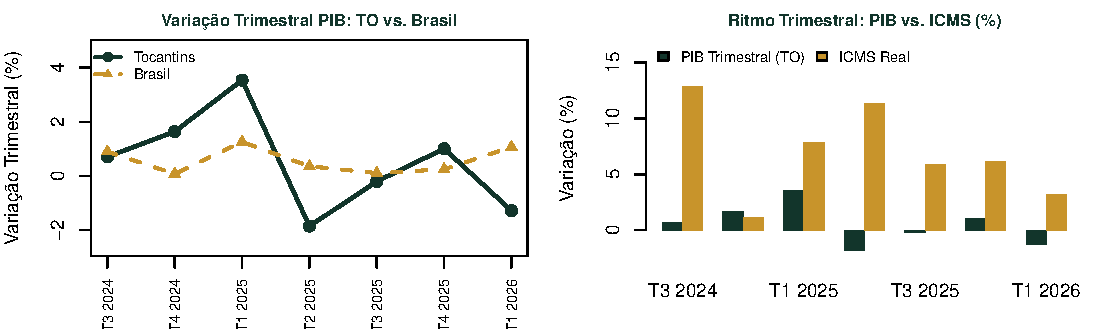
\includegraphics[width=0.98\linewidth]{boletins/build/fig_2026_10_carta_pib.pdf}
\end{center}
\vspace{1pt}
\noindent\begin{minipage}{\linewidth}
{\footnotesize
\noindent\textbf{\textcolor{corprimaria}{Tabela 1 — Desempenho Comparado do Índice de Volume do PIB: Tocantins vs. Brasil (Base 2015 = 100)}}\\[2pt]
\begin{tabularx}{\linewidth}{@{}l X r r r r@{}}
\toprule
\rowcolor{corprimaria} \textcolor{white}{\textbf{Ano}} & \textcolor{white}{\textbf{Índice PIB TO}} & \textcolor{white}{\textbf{Var. Anual TO}} & \textcolor{white}{\textbf{Índice PIB BR}} & \textcolor{white}{\textbf{Var. Anual BR}} & \textcolor{white}{\textbf{Diferencial (TO - BR)}} \\
\midrule
T4 2024 & 2 & +131,0\% & 0 & -91,1\% & +2 pts \\
T1 2025 & 4 & +115,9\% & 1 & +1.475,0\% & +2 pts \\
T2 2025 & -2 & -152,3\% & 0 & -71,4\% & +-2 pts \\
T3 2025 & 0 & -89,2\% & 0 & -69,4\% & +0 pts \\
T4 2025 & 1 & -605,0\% & 0 & +127,3\% & +1 pts \\
T1 2026 & -1 & -226,7\% & 1 & +328,0\% & +-2 pts \\
\bottomrule
\end{tabularx}
}
\end{minipage}
\vspace{2pt}

  }%
}

\vfill
\noindent{\color{douradoto}\rule{\textwidth}{1pt}}\\[-2pt]
{\scriptsize\textcolor{cinzasuave}{\textbf{Expediente e Nota Metodológica:} Instituto Brasileiro de Geografia e Estatística (Sistema de Contas Regionais / IBGE), SEPLAN-TO e Banco Central do Brasil. Elaboração: Jornal Econômico do Tocantins. Publicação diagramada em formato de periódico (2 colunas) pelo Sistema Editorial Híbrido (R + LaTeX) do Jornal Econômico do Tocantins.}}

\end{document}
